% This is the Reed College LaTeX thesis template. Most of the work
% for the document class was done by Sam Noble (SN), as well as this
% template. Later comments etc. by Ben Salzberg (BTS). Additional
% restructuring and APA support by Jess Youngberg (JY).
% Your comments and suggestions are more than welcome; please email
% them to cus@reed.edu
%
% See https://www.reed.edu/cis/help/LaTeX/index.html for help. There are a
% great bunch of help pages there, with notes on
% getting started, bibtex, etc. Go there and read it if you're not
% already familiar with LaTeX.
%
% Any line that starts with a percent symbol is a comment.
% They won't show up in the document, and are useful for notes
% to yourself and explaining commands.
% Commenting also removes a line from the document;
% very handy for troubleshooting problems. -BTS

% As far as I know, this follows the requirements laid out in
% the 2002-2003 Senior Handbook. Ask a librarian to check the
% document before binding. -SN

%%
%% Preamble
%%
% \documentclass{<something>} must begin each LaTeX document
\documentclass[12pt,twoside]{reedthesis}
% Packages are extensions to the basic LaTeX functions. Whatever you
% want to typeset, there is probably a package out there for it.
% Chemistry (chemtex), screenplays, you name it.
% Check out CTAN to see: https://www.ctan.org/
%%
\usepackage{graphicx,latexsym}
\usepackage{amsmath}
\usepackage{amssymb,amsthm}
\usepackage{longtable,booktabs,setspace}
\usepackage{chemarr} %% Useful for one reaction arrow, useless if you're not a chem major
\usepackage[hyphens]{url}
% Added by CII
\usepackage{hyperref}
\usepackage{lmodern}
\usepackage{float}
\floatplacement{figure}{H}
% Thanks, @Xyv
\usepackage{calc}
% End of CII addition
\usepackage{rotating}

% Next line commented out by CII
%%% \usepackage{natbib}
% Comment out the natbib line above and uncomment the following two lines to use the new
% biblatex-chicago style, for Chicago A. Also make some changes at the end where the
% bibliography is included.
%\usepackage{biblatex-chicago}
%\bibliography{thesis}


% Added by CII (Thanks, Hadley!)
% Use ref for internal links
\renewcommand{\hyperref}[2][???]{\autoref{#1}}
\def\chapterautorefname{Chapter}
\def\sectionautorefname{Section}
\def\subsectionautorefname{Subsection}
% End of CII addition

% Added by CII
\usepackage{caption}
\captionsetup{width=5in}
% End of CII addition

% \usepackage{times} % other fonts are available like times, bookman, charter, palatino

% Syntax highlighting #22
  \usepackage{color}
  \usepackage{fancyvrb}
  \newcommand{\VerbBar}{|}
  \newcommand{\VERB}{\Verb[commandchars=\\\{\}]}
  \DefineVerbatimEnvironment{Highlighting}{Verbatim}{commandchars=\\\{\}}
  % Add ',fontsize=\small' for more characters per line
  \usepackage{framed}
  \definecolor{shadecolor}{RGB}{248,248,248}
  \newenvironment{Shaded}{\begin{snugshade}}{\end{snugshade}}
  \newcommand{\AlertTok}[1]{\textcolor[rgb]{0.94,0.16,0.16}{#1}}
  \newcommand{\AnnotationTok}[1]{\textcolor[rgb]{0.56,0.35,0.01}{\textbf{\textit{#1}}}}
  \newcommand{\AttributeTok}[1]{\textcolor[rgb]{0.77,0.63,0.00}{#1}}
  \newcommand{\BaseNTok}[1]{\textcolor[rgb]{0.00,0.00,0.81}{#1}}
  \newcommand{\BuiltInTok}[1]{#1}
  \newcommand{\CharTok}[1]{\textcolor[rgb]{0.31,0.60,0.02}{#1}}
  \newcommand{\CommentTok}[1]{\textcolor[rgb]{0.56,0.35,0.01}{\textit{#1}}}
  \newcommand{\CommentVarTok}[1]{\textcolor[rgb]{0.56,0.35,0.01}{\textbf{\textit{#1}}}}
  \newcommand{\ConstantTok}[1]{\textcolor[rgb]{0.00,0.00,0.00}{#1}}
  \newcommand{\ControlFlowTok}[1]{\textcolor[rgb]{0.13,0.29,0.53}{\textbf{#1}}}
  \newcommand{\DataTypeTok}[1]{\textcolor[rgb]{0.13,0.29,0.53}{#1}}
  \newcommand{\DecValTok}[1]{\textcolor[rgb]{0.00,0.00,0.81}{#1}}
  \newcommand{\DocumentationTok}[1]{\textcolor[rgb]{0.56,0.35,0.01}{\textbf{\textit{#1}}}}
  \newcommand{\ErrorTok}[1]{\textcolor[rgb]{0.64,0.00,0.00}{\textbf{#1}}}
  \newcommand{\ExtensionTok}[1]{#1}
  \newcommand{\FloatTok}[1]{\textcolor[rgb]{0.00,0.00,0.81}{#1}}
  \newcommand{\FunctionTok}[1]{\textcolor[rgb]{0.00,0.00,0.00}{#1}}
  \newcommand{\ImportTok}[1]{#1}
  \newcommand{\InformationTok}[1]{\textcolor[rgb]{0.56,0.35,0.01}{\textbf{\textit{#1}}}}
  \newcommand{\KeywordTok}[1]{\textcolor[rgb]{0.13,0.29,0.53}{\textbf{#1}}}
  \newcommand{\NormalTok}[1]{#1}
  \newcommand{\OperatorTok}[1]{\textcolor[rgb]{0.81,0.36,0.00}{\textbf{#1}}}
  \newcommand{\OtherTok}[1]{\textcolor[rgb]{0.56,0.35,0.01}{#1}}
  \newcommand{\PreprocessorTok}[1]{\textcolor[rgb]{0.56,0.35,0.01}{\textit{#1}}}
  \newcommand{\RegionMarkerTok}[1]{#1}
  \newcommand{\SpecialCharTok}[1]{\textcolor[rgb]{0.00,0.00,0.00}{#1}}
  \newcommand{\SpecialStringTok}[1]{\textcolor[rgb]{0.31,0.60,0.02}{#1}}
  \newcommand{\StringTok}[1]{\textcolor[rgb]{0.31,0.60,0.02}{#1}}
  \newcommand{\VariableTok}[1]{\textcolor[rgb]{0.00,0.00,0.00}{#1}}
  \newcommand{\VerbatimStringTok}[1]{\textcolor[rgb]{0.31,0.60,0.02}{#1}}
  \newcommand{\WarningTok}[1]{\textcolor[rgb]{0.56,0.35,0.01}{\textbf{\textit{#1}}}}

% To pass between YAML and LaTeX the dollar signs are added by CII
\title{Computational analysis of multi-omics data to understand the molecular mechanisms of germline-dependent epigenetic inheritance}
\author{Deepak Kumar Tanwar}
% The month and year that you submit your FINAL draft TO THE LIBRARY (May or December)
\date{}
\division{}
\advisor{}
\institution{ETH Zurich}
\degree{}
%If you have two advisors for some reason, you can use the following
% Uncommented out by CII
% End of CII addition

%%% Remember to use the correct department!
\department{}
% if you're writing a thesis in an interdisciplinary major,
% uncomment the line below and change the text as appropriate.
% check the Senior Handbook if unsure.
%\thedivisionof{The Established Interdisciplinary Committee for}
% if you want the approval page to say "Approved for the Committee",
% uncomment the next line
%\approvedforthe{Committee}

% Added by CII
%%% Copied from knitr
%% maxwidth is the original width if it's less than linewidth
%% otherwise use linewidth (to make sure the graphics do not exceed the margin)
\makeatletter
\def\maxwidth{ %
  \ifdim\Gin@nat@width>\linewidth
    \linewidth
  \else
    \Gin@nat@width
  \fi
}
\makeatother

% From {rticles}
\newlength{\csllabelwidth}
\setlength{\csllabelwidth}{3em}
\newlength{\cslhangindent}
\setlength{\cslhangindent}{1.5em}
% for Pandoc 2.8 to 2.10.1
\newenvironment{cslreferences}%
  {}%
  {\par}
% For Pandoc 2.11+
% As noted by @mirh [2] is needed instead of [3] for 2.12
\newenvironment{CSLReferences}[2] % #1 hanging-ident, #2 entry spacing
 {% don't indent paragraphs
  \setlength{\parindent}{0pt}
  % turn on hanging indent if param 1 is 1
  \ifodd #1 \everypar{\setlength{\hangindent}{\cslhangindent}}\ignorespaces\fi
  % set entry spacing
  \ifnum #2 > 0
  \setlength{\parskip}{#2\baselineskip}
  \fi
 }%
 {}
\usepackage{calc} % for calculating minipage widths
\newcommand{\CSLBlock}[1]{#1\hfill\break}
\newcommand{\CSLLeftMargin}[1]{\parbox[t]{\csllabelwidth}{#1}}
\newcommand{\CSLRightInline}[1]{\parbox[t]{\linewidth - \csllabelwidth}{#1}}
\newcommand{\CSLIndent}[1]{\hspace{\cslhangindent}#1}

\renewcommand{\contentsname}{Table of Contents}
% End of CII addition

\setlength{\parskip}{0pt}

% Added by CII

\providecommand{\tightlist}{%
  \setlength{\itemsep}{0pt}\setlength{\parskip}{0pt}}

\Acknowledgements{
I want to thank a few people.
}

\Dedication{

}

\Preface{

}

\Abstract{

}

	\usepackage{setspace}\onehalfspacing
 \usepackage{acronym}
 \usepackage{glossaries}
 \usepackage{biblatex}
 \usepackage{fancyhdr}
 \usepackage{graphics}
 \usepackage{float}
 \usepackage{placeins}
 \usepackage{lmodern}
% End of CII addition
%%
%% End Preamble
%%
%
\begin{document}

% Everything below added by CII
  \maketitle

\frontmatter % this stuff will be roman-numbered
\pagestyle{empty} % this removes page numbers from the frontmatter
  \begin{acknowledgements}
    I want to thank a few people.
  \end{acknowledgements}

  \hypersetup{linkcolor=black}
  \setcounter{secnumdepth}{2}
  \setcounter{tocdepth}{2}
  \tableofcontents

  \listoftables

  \listoffigures



\mainmatter % here the regular arabic numbering starts
\pagestyle{fancyplain} % turns page numbering back on

\hypertarget{list-of-abbreviations}{%
\chapter*{List of Abbreviations}\label{list-of-abbreviations}}
\addcontentsline{toc}{chapter}{List of Abbreviations}
\begin{acronym}[MPC]
\acro{MPC}{model predictive control}
\acro{TLA}{Three Letter Acronym}
\end{acronym}
\hypertarget{abstract}{%
\chapter*{Abstract}\label{abstract}}
\addcontentsline{toc}{chapter}{Abstract}

\hypertarget{abstract-de}{%
\chapter*{Zusammenfassung}\label{abstract-de}}
\addcontentsline{toc}{chapter}{Zusammenfassung}

\hypertarget{intro}{%
\chapter*{Introduction}\label{intro}}
\addcontentsline{toc}{chapter}{Introduction}

\hypertarget{epigenetics}{%
\section{Epigenetics}\label{epigenetics}}

\hypertarget{germline-epigenetics}{%
\section{Germline epigenetics}\label{germline-epigenetics}}

\hypertarget{spermatogonial-stem-cells}{%
\subsection{Spermatogonial Stem Cells}\label{spermatogonial-stem-cells}}

\hypertarget{reprogramming}{%
\subsection{Reprogramming}\label{reprogramming}}

\hypertarget{epigenetic-inheritance}{%
\section{Epigenetic Inheritance}\label{epigenetic-inheritance}}

\hypertarget{transgenerational-epigenetic-inheritance}{%
\subsection{Transgenerational Epigenetic Inheritance}\label{transgenerational-epigenetic-inheritance}}

\hypertarget{models-of-epigenetic-inheritance}{%
\section{Models of Epigenetic Inheritance}\label{models-of-epigenetic-inheritance}}

\hypertarget{msus-mouse-model}{%
\subsection{MSUS mouse model}\label{msus-mouse-model}}

\hypertarget{vectors-of-tei}{%
\section{Vectors of TEI}\label{vectors-of-tei}}

\hypertarget{extracellular-vesicles}{%
\subsection{Extracellular vesicles}\label{extracellular-vesicles}}

\hypertarget{small-rnas}{%
\subsection{Small RNAs}\label{small-rnas}}

\hypertarget{methods}{%
\chapter*{Bioinformatics methods}\label{methods}}
\addcontentsline{toc}{chapter}{Bioinformatics methods}

\hypertarget{version-controlled-data-analysis-using-git}{%
\section{Version controlled data analysis using git}\label{version-controlled-data-analysis-using-git}}

\hypertarget{data-analysis-directory-organization}{%
\section{Data analysis directory organization}\label{data-analysis-directory-organization}}

\hypertarget{pipelines-for-data-analysis}{%
\section{Pipelines for data analysis}\label{pipelines-for-data-analysis}}

\hypertarget{bulk-rna-seq}{%
\subsection{Bulk RNA-seq}\label{bulk-rna-seq}}

\hypertarget{atac-seq}{%
\subsection{ATAC-seq}\label{atac-seq}}

\hypertarget{chip-seq}{%
\subsection{ChIP-seq}\label{chip-seq}}

\hypertarget{wgbs-rrbs}{%
\subsection{WGBS \& RRBS}\label{wgbs-rrbs}}

\hypertarget{small-rna-seq}{%
\subsection{small RNA-seq}\label{small-rna-seq}}

\hypertarget{challenges-for-analyzing-srna-seq-dataset}{%
\subsubsection{Challenges for analyzing sRNA-seq dataset}\label{challenges-for-analyzing-srna-seq-dataset}}

\hypertarget{aims}{%
\chapter*{Aims and thesis overview}\label{aims}}
\addcontentsline{toc}{chapter}{Aims and thesis overview}

\hypertarget{aims-1}{%
\section{Aims}\label{aims-1}}

\hypertarget{thesis-overview}{%
\section{Thesis overview}\label{thesis-overview}}

\hypertarget{developmental}{%
\chapter{Dynamic chromatin accessibility in spermatogonial cells for transcriptional programmings from early postnatal to adult stages}\label{developmental}}

\newpage

\hypertarget{graphical-abstract}{%
\section{Graphical Abstract}\label{graphical-abstract}}

\newpage

\hypertarget{abstract-1}{%
\section{Abstract}\label{abstract-1}}

\newpage

\hypertarget{introduction}{%
\section{Introduction}\label{introduction}}

\newpage

\hypertarget{results}{%
\section{Results}\label{results}}

\hypertarget{enrichment-of-spermatogonial-cells-from-postnatal-and-adult-mouse-testis}{%
\subsection{Enrichment of spermatogonial cells from postnatal and adult mouse testis}\label{enrichment-of-spermatogonial-cells-from-postnatal-and-adult-mouse-testis}}

\hypertarget{chromatin-is-remodeled-in-spermatogonial-cells-during-development}{%
\subsection{Chromatin is remodeled in spermatogonial cells during development}\label{chromatin-is-remodeled-in-spermatogonial-cells-during-development}}

\hypertarget{differentially-accessible-chromatin-regions-associate-with-distinct-gene-expression-dynamics}{%
\subsection{Differentially accessible chromatin regions associate with distinct gene expression dynamics}\label{differentially-accessible-chromatin-regions-associate-with-distinct-gene-expression-dynamics}}

\hypertarget{differentially-accessible-chromatin-regions-associate-with-distinct-epigenetic-profiles}{%
\subsection{Differentially accessible chromatin regions associate with distinct epigenetic profiles}\label{differentially-accessible-chromatin-regions-associate-with-distinct-epigenetic-profiles}}

\hypertarget{accessibility-changes-at-open-chromatin-regions-are-markedcarry-by-binding-sites-for-distinct-families-of-transcription-factors}{%
\subsection{Accessibility changes at open chromatin regions are markedcarry by binding sites for distinct families of transcription factors}\label{accessibility-changes-at-open-chromatin-regions-are-markedcarry-by-binding-sites-for-distinct-families-of-transcription-factors}}

\hypertarget{chromatin-accessibility-at-transposable-elements-undergoes-significant-remodeling-in-the-transition-from-postnatal-to-adult-spermatogonia}{%
\subsection{Chromatin accessibility at transposable elements undergoes significant remodeling in the transition from postnatal to adult spermatogonia}\label{chromatin-accessibility-at-transposable-elements-undergoes-significant-remodeling-in-the-transition-from-postnatal-to-adult-spermatogonia}}

\newpage

\hypertarget{discussion}{%
\section{Discussion}\label{discussion}}

\newpage

\hypertarget{methods-1}{%
\section{Methods}\label{methods-1}}

\hypertarget{mouse-husbandry}{%
\subsection{Mouse husbandry}\label{mouse-husbandry}}

\hypertarget{germ-cells-isolation}{%
\subsection{Germ cells isolation}\label{germ-cells-isolation}}

\hypertarget{spermatogonial-cells-enrichment-by-facs}{%
\subsection{Spermatogonial cells enrichment by FACS}\label{spermatogonial-cells-enrichment-by-facs}}

\hypertarget{immunocytochemistry}{%
\subsection{Immunocytochemistry}\label{immunocytochemistry}}

\hypertarget{rna-extraction-and-rna-seq-library-preparation-for-rna-seq}{%
\subsection{RNA extraction and RNA-seq library preparation for RNA-seq}\label{rna-extraction-and-rna-seq-library-preparation-for-rna-seq}}

\hypertarget{omni-atac-llibrary-preparation-for-omni-atac-and-sequencing}{%
\subsection{Omni-ATAC Llibrary preparation for Omni-ATAC and sequencing}\label{omni-atac-llibrary-preparation-for-omni-atac-and-sequencing}}

\hypertarget{rna-sequencing-rna-seq}{%
\subsection{RNA sequencing (RNA-seq)}\label{rna-sequencing-rna-seq}}

\hypertarget{assay-for-transposase-accessible-chromatin-using-sequening-omni-atac}{%
\subsection{Assay for Transposase-Accessible Chromatin using sequening (Omni-ATAC)}\label{assay-for-transposase-accessible-chromatin-using-sequening-omni-atac}}

\hypertarget{chromatin-iimmunnoprecipitation-sequencing-chip-seq}{%
\subsection{Chromatin iImmunnoprecipitation sequencing (ChIP-seq)}\label{chromatin-iimmunnoprecipitation-sequencing-chip-seq}}

\hypertarget{bisulfite-sequencing-bs}{%
\subsection{Bisulfite sequencing (BS)}\label{bisulfite-sequencing-bs}}

\hypertarget{high-throughput-sequencing-data-analysis}{%
\subsection{High-throughput sequencing data analysis}\label{high-throughput-sequencing-data-analysis}}

\hypertarget{figures}{%
\subsection{Figures}\label{figures}}

\newpage

\hypertarget{data-and-materials-availability}{%
\section{Data and materials availability}\label{data-and-materials-availability}}

\hypertarget{authors-contribution}{%
\section{Authors Contribution}\label{authors-contribution}}

\hypertarget{competing-interest}{%
\section{Competing interest}\label{competing-interest}}

\newpage

\hypertarget{acknowledgments}{%
\section{Acknowledgments}\label{acknowledgments}}

\hypertarget{funding}{%
\section{Funding}\label{funding}}

\newpage

\hypertarget{supplementary-figures}{%
\section{Supplementary Figures}\label{supplementary-figures}}

\hypertarget{figure-1}{%
\subsection{Figure 1}\label{figure-1}}

\hypertarget{figure-2}{%
\subsection{Figure 2}\label{figure-2}}

\hypertarget{figure-3}{%
\subsection{Figure 3}\label{figure-3}}

\hypertarget{figure-4}{%
\subsection{Figure 4}\label{figure-4}}

\hypertarget{figure-5}{%
\subsection{Figure 5}\label{figure-5}}

\hypertarget{figure-6}{%
\subsection{Figure 6}\label{figure-6}}

\newpage

\hypertarget{references}{%
\section{References}\label{references}}

\hypertarget{ev}{%
\chapter{Early life stress affects the miRNA cargo of epididymal extracellular vesicles in mouse}\label{ev}}

Anar Alshanbayeva\textsuperscript{1,2,3}, \textbf{Deepak K Tanwar}\textsuperscript{1,2,3}, Martin Roszkowski\textsuperscript{1,2,3}, Francesca Manuella\textsuperscript{1,2,3}, Isabelle M Mansuy\textsuperscript{1,2,3,\#}
\newline
\newline
\textsuperscript{1}Laboratory of Neuroepigenetics, Brain Research Institute at the Medical Faculty of the University of Zurich.
\newline
\textsuperscript{2}Institute for Neuroscience of the Department of Health Sciences and Technology, ETH Zurich, Zurich, Switzerland.
\newline
\textsuperscript{3}Zurich Neuroscience Center, ETH and University of Zurich, Zurich, Switzerland.
\newline
\newline
\textsuperscript{\#}Corresponding author
\newline
\newline
\textbf{Journal:} \emph{Biology of Reproduction}
\newline
DOI: \href{https://doi.org/10.1093/biolre/ioab156}{10.1093/biolre/ioab156}
\newline
\newline
\textbf{Contributions:} \emph{I performed data analysis with Anar Alshanbayeva, generated figures with Anar Alshanbayeva, helped Anar Alshanbayeva in writing the manuscript, and revised manuscript with Anar Alshanbayeva.}

\newpage

\hypertarget{abstract-2}{%
\section{Abstract}\label{abstract-2}}

Sperm RNA can be modified by environmental factors and has been implicated in communicating signals about changes in a father's environment to the offspring. The small RNA composition of sperm could be changed during its final stage of maturation in the epididymis by extracellular vesicles (EVs) released by epididymal cells. We studied the effect of exposure to stress in early postnatal life on the transcriptome of epididymal EVs using a mouse model of transgenerational transmission. We found that the small RNA signature of epididymal EVs, particularly miRNAs, is altered in adult males exposed to postnatal stress. In some cases, these miRNA changes correlate with differences in the expression of their target genes in sperm and zygotes generated from that sperm. These results suggest that stressful experiences in early life can have persistent biological effects on the male reproductive tract that may in part be responsible for the transmission of the effects of exposure to the offspring.

\hypertarget{summary-sentence}{%
\section{Summary sentence}\label{summary-sentence}}

miRNA cargo of extracellular vesicles in cauda epididymis is altered by paternal exposure to early life stress. This correlates with changes in the expression of target genes in sperm and in zygotes generated from that sperm.

\newpage

\hypertarget{graphical-abstract-1}{%
\section{Graphical Abstract}\label{graphical-abstract-1}}

\hypertarget{key-words}{%
\section{Key words}\label{key-words}}

epigenetics, epididymis, epididymosomes, early life stress, extracellular vesicles, miRNAs, sperm.

\newpage

\hypertarget{introduction-1}{%
\section{Introduction}\label{introduction-1}}

Post-testicular maturation of spermatozoa in the epididymis is an elaborate process that involves modifications of sperm RNA, protein, and lipid content (Nixon et al., 2015; Rejraji et al., 2006; Sharma et al., 2016; Skerget, Rosenow, Petritis, \& Karr, 2015; Tamessar et al., 2021). The epididymis is segmented into different parts, including the initial segment, caput, corpus, and cauda. Each segment has a distinct gene expression profile, and different protein and lipid composition. Some modifications in epididymal spermatozoa are conserved across species (Sellem et al., 2020). For example, \textasciitilde50\% of miRNAs, a class of small RNAs that are modified during caput to cauda epididymis transit, is identical in mouse and bovine spermatozoa (Sellem et al., 2020). One mechanism by which small RNA load in spermatozoa is modified along the epididymis is by uptake of extracellular vesicles (EVs), also known as epididymosomes, which are produced by epididymal epithelial cells (Reilly et al., 2016). Studies have shown that epididymosomes can be taken up by maturing sperm through proteins present on the sperm head such as dynamin in mice and tetraspanins or syntenins in humans (Caballero, Frenette, Belleannée, \& Sullivan, 2013; Reilly et al., 2016; Thimon, Frenette, Saez, Thabet, \& Sullivan, 2008; Zhou et al., 2019). Co-incubation experiments provided evidence for epididymosome-mediated transfer of miRNAs to spermatozoa (Reilly et al., 2016). Exogenous DNA and RNA can also be directly taken up by spermatozoa via artificial liposomes (Bachiller, Schellander, Peli, \& Rüther, 1991).

However, it is still not clear if changes in small RNA composition of spermatozoa occurring during epididymal transit are required for embryonic development, and studies on the subject have been conflicting (Conine, Sun, Song, Rivera-Pérez, \& Rando, 2018; Suganuma, Yanagimachi, \& Meistrich, 2005). Changes in sperm small RNA have nevertheless been suggested to play a role in the transmission of information about paternal experiences to the progeny and can influence their developmental trajectory (Chan et al., 2020; Katharina Gapp et al., 2014; Sharma et al., 2016). Epididymosomal small RNA content can also be altered by exposure, for instance, to dietary insult and stress (Chan et al., 2020; Sharma et al., 2016). For instance, epididymosomal miRNAs are changed by exposure to chronic stress (Chan et al., 2020) and low-protein diet (Sharma et al., 2016) in mice.

Transmission of information about paternal exposure to the offspring depends on the type of exposure, its duration and the developmental window at which it is applied. To date, little is known about the long-term effects of early life stress, particularly stress experienced after birth, on epididymosomal small RNA composition in adulthood, and whether any changes to this composition can influence gene expression in sperm and in zygotes generated from that sperm. Using a transgenerational mouse model of postnatal stress induced by unpredictable maternal separation combined with unpredictable maternal stress, unpredictable maternal separation combined with unpredictable maternal stress (MSUS) (Franklin et al., 2010), we show that the miRNA signature of cauda epididymosomes in adult males is altered by exposure, and that this alteration, correlates with changes in the expression of their target genes in sperm and in zygotes.

\newpage

\hypertarget{results-1}{%
\section{Results}\label{results-1}}

\hypertarget{isolation-of-cauda-epididymosomes-confirmed-by-several-methods}{%
\subsection{Isolation of cauda epididymosomes confirmed by several methods}\label{isolation-of-cauda-epididymosomes-confirmed-by-several-methods}}
\begin{figure}

{\centering 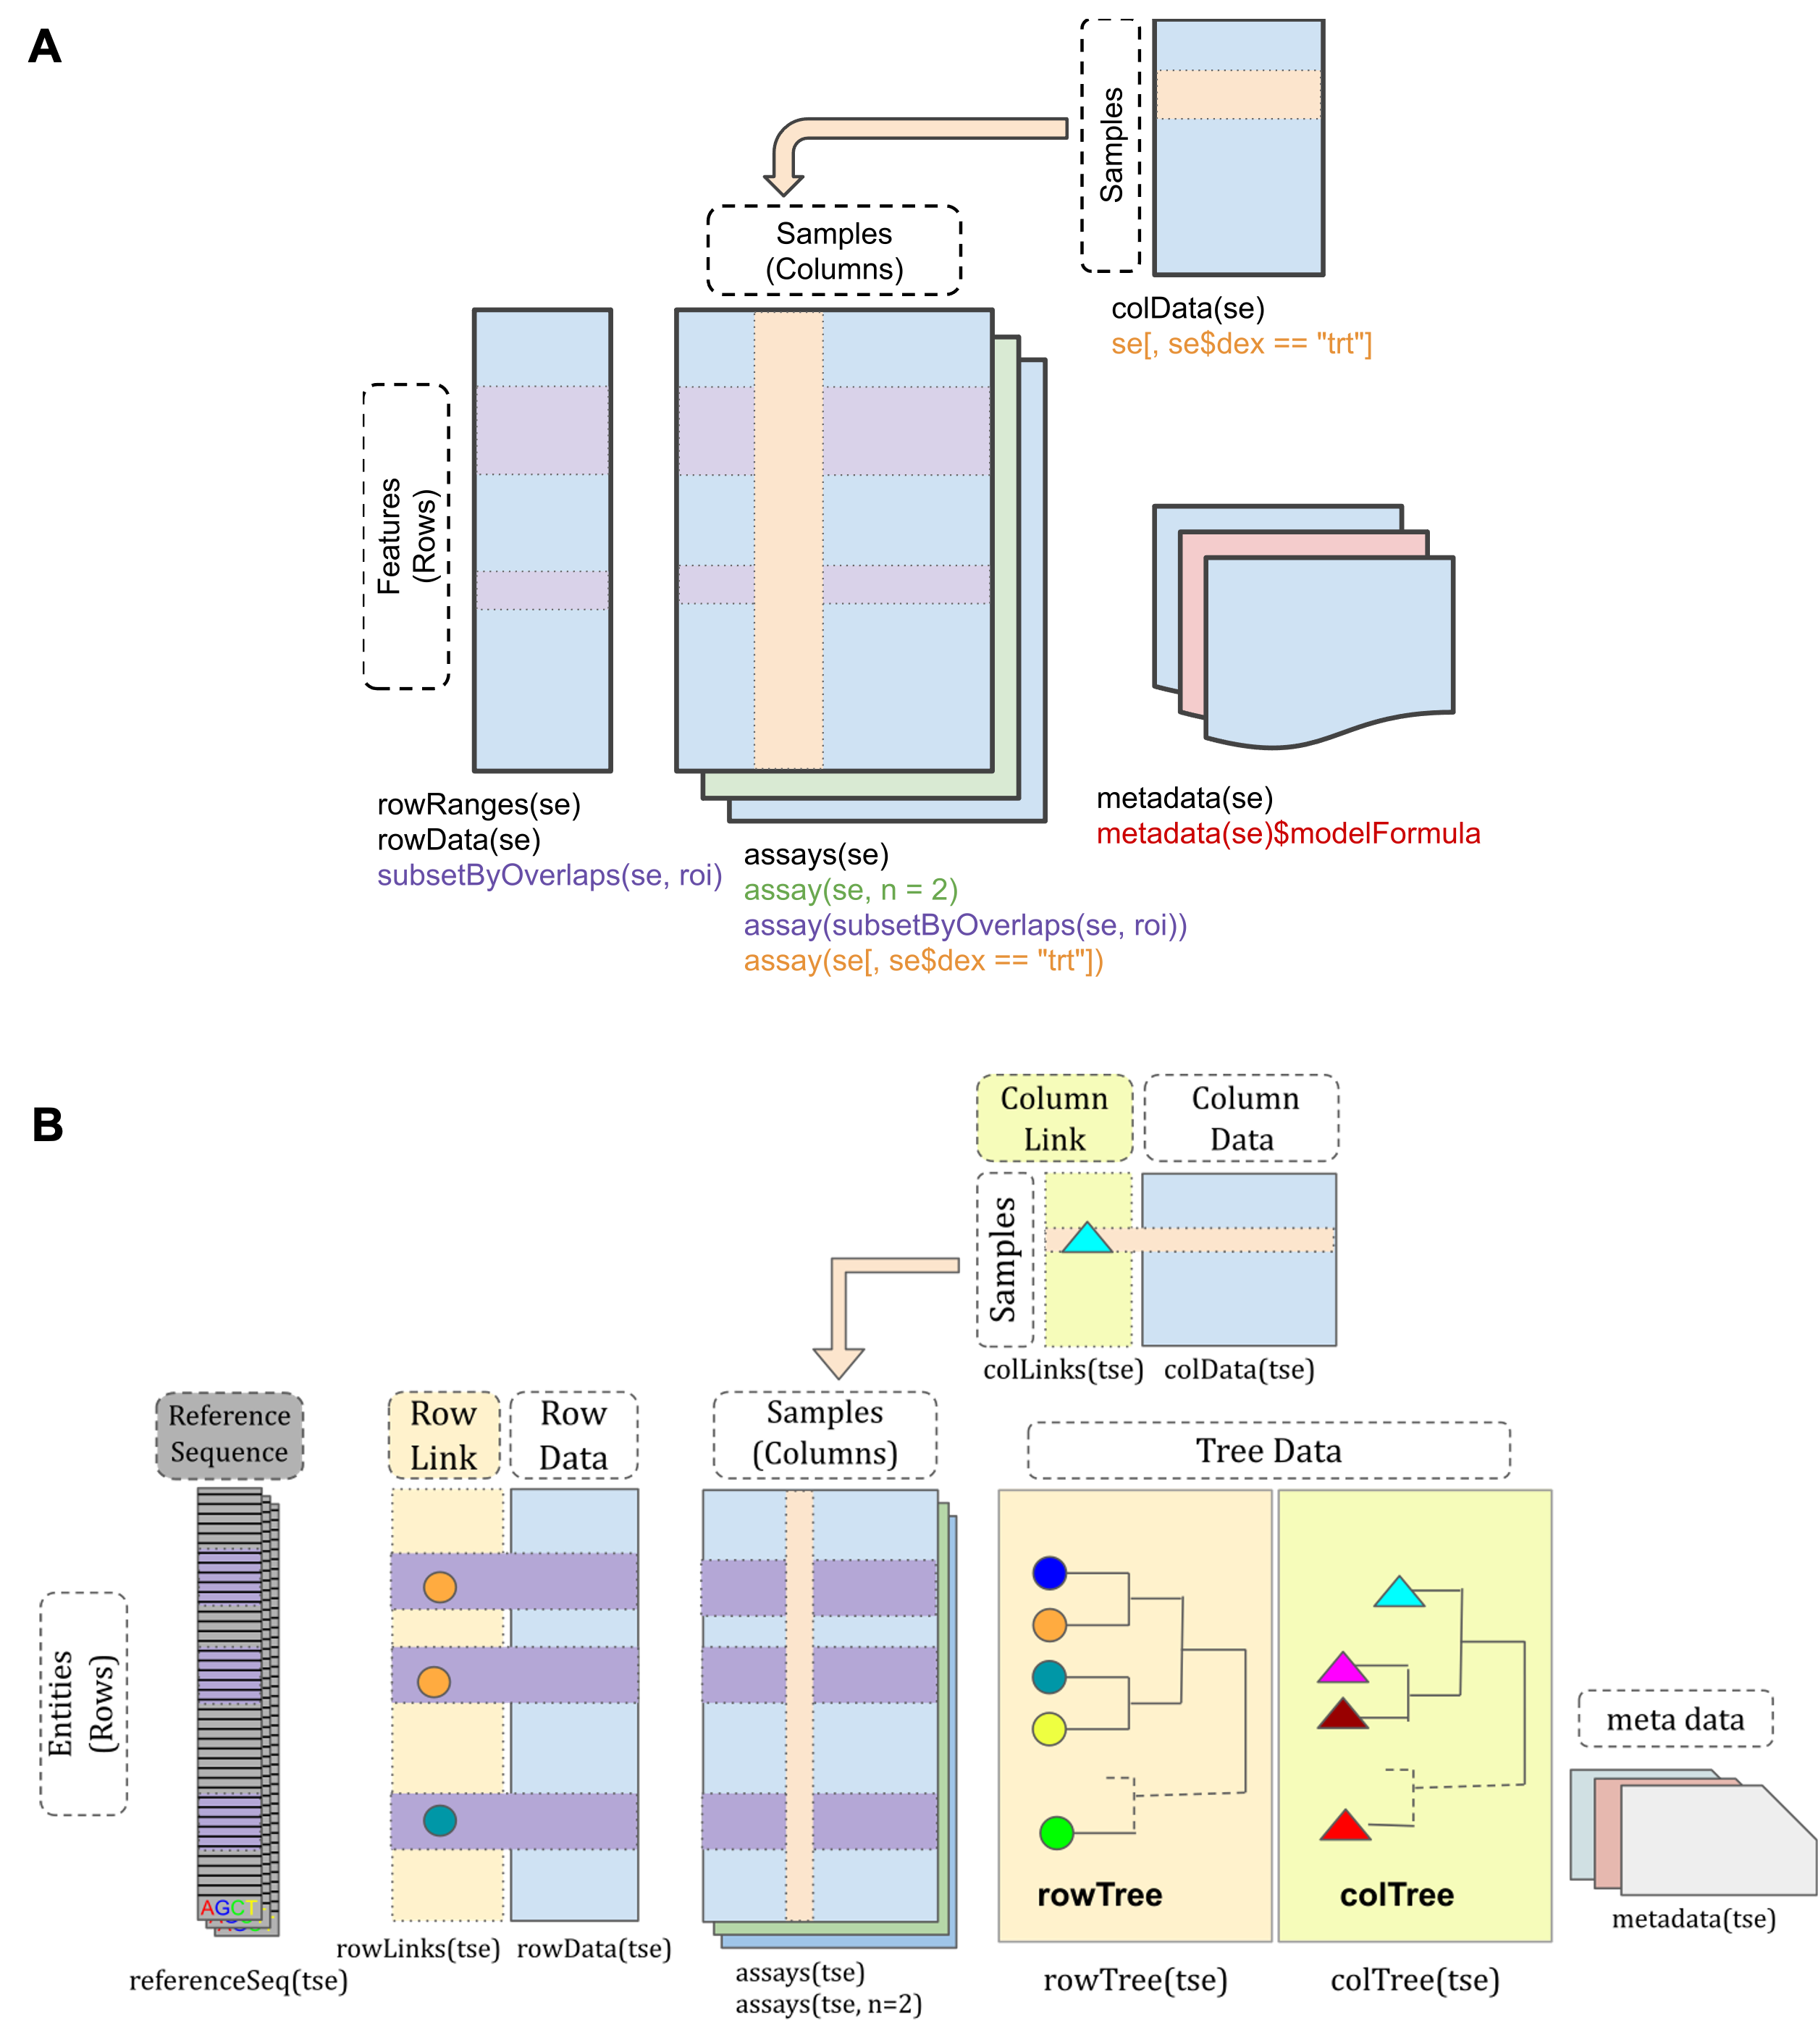
\includegraphics{figure/1} 

}

\caption{testFig}\label{fig:fig1}
\end{figure}
\ref{fig:fig1} is a figure
\begin{Shaded}
\begin{Highlighting}[]
\NormalTok{df }\OtherTok{\textless{}{-}} \FunctionTok{matrix}\NormalTok{(}\AttributeTok{data =} \FunctionTok{rnorm}\NormalTok{(}\DecValTok{100}\NormalTok{, }\DecValTok{1}\NormalTok{,}\DecValTok{1}\NormalTok{), }\AttributeTok{nrow =} \DecValTok{10}\NormalTok{)}
\NormalTok{knitr}\SpecialCharTok{::}\FunctionTok{kable}\NormalTok{(df,}\AttributeTok{label =} \StringTok{"tab1"}\NormalTok{,}
  \AttributeTok{caption =} \StringTok{"Maximum Delays by Airline"}\NormalTok{,}
  \AttributeTok{caption.short =} \StringTok{"Max Delays by Airline"}\NormalTok{,}
  \AttributeTok{longtable =} \ConstantTok{TRUE}\NormalTok{,}
  \AttributeTok{booktabs =} \ConstantTok{TRUE}
\NormalTok{)}
\end{Highlighting}
\end{Shaded}
\begin{longtable}[t]{rrrrrrrrrr}
\caption[Max Delays by Airline]{\label{tab:tab1}Maximum Delays by Airline}\\
\toprule
2.5675662 & 1.8994650 & 0.5984832 & 1.4550607 & 0.2674034 & -0.7039193 & 0.2960841 & 2.7584654 & 2.1186707 & 1.9721139\\
1.6178904 & -0.2893781 & 0.3917197 & 0.7800107 & -0.6885410 & 0.7339272 & 3.3245881 & 1.5900233 & 2.1839153 & 0.5537705\\
2.5700141 & 2.5185762 & 0.6249687 & 2.2810414 & 0.9081730 & 2.3136164 & -0.0020126 & 0.9984115 & 0.6162636 & 1.9532397\\
0.1697651 & -0.4551171 & 1.3036652 & 1.4137001 & 0.8357247 & 2.8430917 & 1.4120191 & 1.9655317 & 1.5081944 & 1.0197923\\
1.6607558 & 0.2319071 & 1.7488949 & 2.5355426 & -0.7098591 & 0.9707308 & 0.7522115 & 0.9151569 & 1.9428591 & 1.8152508\\
\addlinespace
1.0153006 & -0.0059650 & -0.6748931 & 1.2601895 & 0.5099000 & 2.1646708 & 0.2852806 & 0.3713330 & 0.7601931 & 0.0321145\\
0.2227486 & -0.1996470 & 1.0743309 & 1.2461758 & 1.6948151 & 1.8507603 & -0.1818836 & 0.6618011 & 0.9277586 & 1.9883086\\
0.8383722 & 0.5456429 & 0.1761501 & 1.3404653 & -0.2389068 & 1.0350949 & 0.8465461 & 0.3928817 & 1.4480509 & -0.9352212\\
1.1289393 & 3.2673492 & -0.6718739 & -0.1991586 & -0.1178724 & 0.6746644 & 1.9637217 & 3.0022748 & 0.2534978 & 0.2832933\\
-0.3786795 & 1.8266442 & -0.4390031 & 1.9302657 & 0.4471014 & 0.7284932 & 0.4261575 & 4.3020458 & -0.2563755 & 1.6971400\\
\bottomrule
\end{longtable}
\ref{tab:tab1} is a table

--\textgreater{}

\hypertarget{the-number-and-size-of-epididymosomes-in-adult-males-are-not-altered-by-postnatal-stress}{%
\subsection{The number and size of epididymosomes in adult males are not altered by postnatal stress}\label{the-number-and-size-of-epididymosomes-in-adult-males-are-not-altered-by-postnatal-stress}}

\hypertarget{mirnas-are-persistently-altered-by-postnatal-stress-in-cauda-epididymosomes}{%
\subsection{miRNAs are persistently altered by postnatal stress in cauda epididymosomes}\label{mirnas-are-persistently-altered-by-postnatal-stress-in-cauda-epididymosomes}}

\hypertarget{mrna-targets-of-mirnas-from-cauda-epididymosomes-are-altered-by-postnatal-stress-in-sperm-and-in-zygotes}{%
\subsection{mRNA targets of miRNAs from cauda epididymosomes are altered by postnatal stress in sperm and in zygotes}\label{mrna-targets-of-mirnas-from-cauda-epididymosomes-are-altered-by-postnatal-stress-in-sperm-and-in-zygotes}}

\newpage

\hypertarget{discussion-1}{%
\section{Discussion}\label{discussion-1}}

The effects of environmental factors on RNA in the male reproductive tract, in particular, the epididymis have been examined in rodent models. Until now, most models have used invasive exposure such as dietary insult or injection of endocrine disruptors, applied prenatally and sometimes before conception. Few studies have examined the effects of non-invasive psychological/emotional exposure such as stress in early life and the effects on epididymal RNA in adulthood (Chan et al., 2020). This study examines if postnatal stress affects RNAs in EVs released from the cauda epididymis and whether this has consequences for mature sperm and zygotes generated from that sperm.

Using a transgenerational mouse model of early postnatal stress, we show that several miRNAs, including miR-871-3p, miR-31-5p, miR-155-5p, miR-878-5p, and miR-34c-5p are altered in cauda epididymosomes in adult males exposed to postnatal stress, and that the targets of some of these miRNAs are affected in mature sperm and zygotes. Particularly, miR-31-5p is significantly decreased in cauda epididymosomes and its target genes are up-regulated in sperm but down-regulated in zygotes generated from that sperm, suggesting an over-compensation during early development. This may also be due to the heterogeneity of epididymosomes which have different size, biogenesis, and cellular targeting (Sullivan, 2015), leading to a dissociation between the RNA content of epididymosomes and transcriptional changes in zygotes. It has been suggested that different subsets of epididymosomes have different roles. While a subset communicates with spermatozoa during sperm epididymal transit (Reilly et al., 2016; Sharma et al., 2016), another subset serves in the communication within epididymal epithelial cells (Belleannée, Calvo, Caballero, \& Sullivan, 2013), and a third one is delivered as part of seminal fluid during fertilization (Belleannée, Légaré, Calvo, Thimon, \& Sullivan, 2013; Frenette, Légaré, Saez, \& Sullivan, 2005). Thus owing to their heterogeneity, not all cauda epididymosomes or their cargo is delivered to the oocyte upon fertilization, which may explain the differences in miRNAs targets that are affected in sperm and zygotes.

Several of the differentially expressed miRNAs in MSUS cauda epididymosomes play a role in metabolic processes and early development (Reza et al., 2019). For instance, miR-31-5p is involved in glucose metabolism and fatty acid oxidation (Reza et al., 2019). In humans, its target complement C1q Tumor Necrosis Factor-Related Protein 9A (CTRP9) protein is negatively correlated with the amount of visceral fat and positively associated with a beneficial glucose and metabolic phenotype (Shao et al., 2017). This is consistent with the observation that glucose and insulin metabolism are also affected by MSUS (Franklin et al., 2010; Katharina Gapp et al., 2014). The level of other miRNAs is significantly increased or decreased in MSUS epididymosomes, such as miR-155-5p, which facilitates differentiation of mouse embryonic stem cells, or miR-34c-5p that initiates the first embryonic cleavage in mice (Reza et al., 2019).

The first days after birth are a sensitive period for the development and the establishment of cellular niches in tissues. Epithelial cells in the epididymis, which are the source of epididymosomes, undergo differentiation and expansion postnatally until puberty (Robaire, Hinton, \& Orgebin-Crist, 2002). Once their expansion is completed, epididymal epithelial cells remain at a nearly constant number in adulthood. If they can be modified by prior exposure, they may therefore carry a memory of exposure into adulthood. The postnatal development and differentiation of epididymal epithelial cells primarily depend on testicular signals (Bilińska et al., 2006; Robaire \& Hamzeh, 2011; Robaire et al., 2002; Zhu et al., 2000). Since chronic stress affects the coupling of the hypothalamus--pituitary and hypothalamus--gonadal axes, stress-related decrease in steroidogenesis can profoundly affect the differentiation and expansion of epididymal epithelial cells in early postnatal life. A number of studies have shown the importance of the abundance of androgens during postnatal life for epididymal development (Robaire et al., 2002). Thus, the availability of testicular cholesterol during epididymal cells differentiation has implications for these cells. Systemic alteration in cholesterol metabolism seen in young MSUS males (decreased total cholesterol in testis and increased HDL cholesterol in liver) may contribute to metabolic changes seen in adult animals, for instance in plasma steroidogenesis and fatty acid pathways, and to alterations in glucose and insulin metabolism in adult MSUS males. Moreover, androgen-dependent miRNAs miR-878-5p and miR-871-3p are significantly increased in cauda epididymosomes in MSUS.

In conclusion, our results provide evidence that chronic stress in early postnatal life alters miRNAs in EVs of the male reproductive tract in adulthood, with effects in mature sperm and zygotes. These persistent and intergenerational effects in vivo point to the sensitivity of the reproductive system to stress exposure and the detrimental consequences for descendants. These consequences may differ depending on the time window and severity of paternal stress exposure. Further studies are necessary to more precisely define these effects and the source of vesicles and their cargo miRNAs.

\newpage

\hypertarget{materials-and-methods}{%
\section{Materials and methods}\label{materials-and-methods}}

\hypertarget{animals}{%
\subsection{Animals}\label{animals}}

Animal experiments were conducted according to the Swiss Law for Animal Protection and were approved by the cantonal veterinary office in Zürich under license number 83/2018. C57Bl/6 J mice were obtained from Janvier (France) and bred in-house to generate animals for the experiments. Animals were maintained under a reverse light--dark cycle in a temperature and humidity-controlled environment with constant access to food and water. Nine months old age-matched MSUS and control males were used for small RNA-sequencing (sRNA-seq) of cauda epididymosomes, tissue collection for RT-qPCR, nanoparticle-tracking analysis, and total cholesterol measurements. HDL cholesterol and total cholesterol measurements were performed on MSUS and control males at postnatal day 28. Datasets from previous publication (K. Gapp et al., 2020): caudal sperm RNA-seq was performed on 5-months old males, and zygote RNA-seq was performed on zygotes from 3-months old males.

\hypertarget{msus}{%
\subsection{MSUS}\label{msus}}

To obtain MSUS mice, 3-months old C57Bl/6 J females and their litters were subjected to daily 3 h separation unpredictably and females were exposed to an unpredictable stressor during separation as previously described (Franklin et al., 2010). Control dams and pups were left undisturbed. After weaning at postnatal day 21, pups from different litters were randomly assigned to cages of 4--5 mice, in corresponding treatment groups to avoid litter effects.

\hypertarget{tissue-collection}{%
\subsection{Tissue collection}\label{tissue-collection}}

After decapitation and blood collection, mice were pinned on a dissection board and cleaned with alcohol. Epididymis and testis were excised and separated from surrounding adipose tissue. The epididymis was separated into caput, corpus, and cauda. Cauda was excised with several incisions and sperm collected with a swim-up protocol. The supernatant was collected to isolate epididymosomes. The whole testis and caput epididymis were crushed with stainless steel beads in a tissue crusher in cold PBS, centrifuged at 3000 rcf for 10 min to pellet the tissue and cells and used for total cholesterol and HDL cholesterol measurements.

\hypertarget{electron-microscopy-images}{%
\subsection{Electron microscopy images}\label{electron-microscopy-images}}

Negative staining of cauda epididymosomes was performed with methylcellulose. Briefly, the carrier grid was glow-discharged in plasma for 10 min and washed with a drop of PBS, then incubated in 1\% glutaraldehyde (GA) in water for 5 min and washed with water five times for 2 min each. Afterwards the grid was incubated in 1\% UAc (uranyl acetate) for 5 min and then kept on ice in methylcellulose/UAc (900 ul methylcellulose 2\% and 100 ul 3\% UAc) solution. After incubation with methylcellulose/UAc, the excess liquid was removed by dipping onto a filter paper. The grid was air-dried on ice for 5 min. Imaging was performed with a transmission electron microscope.

\hypertarget{epididymosomes-isolation-by-ultracentrifugation}{%
\subsection{Epididymosomes isolation by ultracentrifugation}\label{epididymosomes-isolation-by-ultracentrifugation}}

After pelleting sperm following the sperm swim-up protocol in M2 medium (Sigma, M7167), the supernatant was centrifuged at 2000 rcf for 10 min, 10 000 rcf for 30 min and then ultracentrifuged at 120 000 rcf at 4 \(^{\circ}\)C for 2 h (TH 64.1 rotor, Thermo Fisher Scientific). The epididymosomal pellet was then washed in PBS at 4 \(^{\circ}\)C and ultracentrifuged at 120 000 rcf at 4 \(^{\circ}\)C for 2 h. The resulting pellet was resuspended in 60 \textmu l of PBS for all downstream analysis.

\hypertarget{immunoblotting}{%
\subsection{Immunoblotting}\label{immunoblotting}}

PBS-resuspended pellet containing epididymosomes was lysed in 10x RIPA buffer for 5 min at 4 \(^{\circ}\)C. Equal amounts of protein were mixed with 4x Laemmli Sample Buffer (Bio-Rad Laboratories, USA) and loaded on 4--20\% Tris-Glycine polyacrylamide gels (Bio-Rad Laboratories, USA). The membranes were blocked in 5\% SureBlock (in Tris-buffer with 0.05\% Tween-20) for 1 h at room temperature and incubated with overnight at 4 \(^{\circ}\)C with primary anti-Cd9 ({[}1:3000; System Biosciences, USA{]} and anti-Gapdh {[}1:5000; Cell Signaling, USA; 14C10{]}) antibodies.

\hypertarget{nanoparticle-tracking-analysis}{%
\subsection{Nanoparticle tracking analysis}\label{nanoparticle-tracking-analysis}}

Particle number and size of epididymosomes were measured using a Nanosight NS300 (Malvern, UK) at 20 \(^{\circ}\)C, according to the manufacturer's instructions and lots were generated using a published method (Dragovic et al., 2011). The following parameters were kept constant for all samples: ``Camera level'' = 14 and ``Detection threshold'' = 7. For measurements with Nanosight, the resuspended pellet from ultracentrifugation was diluted to a 1:1000 concentration.

\hypertarget{rna-isolation-and-epididymosomes-profiling}{%
\subsection{RNA isolation and epididymosomes profiling}\label{rna-isolation-and-epididymosomes-profiling}}

To lyse purified epididymosomes, 33 \textmu l of lysis buffer (6.4 M guanidine HCl, 5\% Tween 20, 5\% Triton, 120 mM EDTA, and 120 mM Tris pH 8.0) per 60 \textmu l of PBS resuspended pellet was added to each sample, together with \textmu l Proteinase K and 3.3 \textmu l water. Samples were incubated at 60 \(^{\circ}\)C for 15 min with shaking. A total of 40 \textmu l water were added and RNA was extracted using Trizol LS protocol, according to the manufacturer's instructions. Profiling of extracted RNA was done using high-resolution automated electrophoresis on a 2100 Bioanalyzer (Agilent, G2939BA), according to instructions for the RNA 6000 Pico Kit (Agilent, 5067-1513) reagent.

\hypertarget{preparation-and-sequencing-of-srna-seq-libraries-from-epididymosomes}{%
\subsection{Preparation and sequencing of sRNA-seq libraries from epididymosomes}\label{preparation-and-sequencing-of-srna-seq-libraries-from-epididymosomes}}

sRNA-seq libraries were prepared using the NEB Next Small RNA-sequencing kit (NEB \#E7300, New England BioLabs), according to the manufacturer's instructions. About 80--90 ng of total RNA per sample was used to prepare the libraries. The same libraries were sequenced before and after size-selection (target peak 150 bp) with the BluePippin System. 200 million reads were obtained for 10 samples, with 125 bp single-stranded read-length on a HiSeq2500 sequencer.

\hypertarget{rt-qpcr}{%
\subsection{RT-qPCR}\label{rt-qpcr}}

For gene expression analysis in caput epididymis, RNA was extracted using the phenol/chloroform extraction method (TRIzol; Thermo Fisher Scientific). Reverse transcription was performed using miScript \RN{2} RT reagents (Qiagen) - HiFlex buffer, and RT qPCR was performed with QuantiTect SYBR (Qiagen) on the Light-Cycler \RN{2} 480 (Roche). All samples were run in cycles as follows: 95 \(^{\circ}\)C for 15 min, 45 cycles of 15 s at 94 \(^{\circ}\)C, 30 s at 55 \(^{\circ}\)C and 30 s at 70 \(^{\circ}\)C, followed by gradual increase of temperature to \(^{\circ}\)C. The endogenous control \textit{Gapdh} was used for normalization. The expression level of genes was analyzed using two-tailed Student's \textit{t}-test.

\hypertarget{cholesterol-measurements}{%
\subsection{Cholesterol measurements}\label{cholesterol-measurements}}

Testicular and epididymal total cholesterol and HDL cholesterol levels were measured using the CHOL reagent, in conjunction with SYNCHRON LX System(s), UniCel DxC 600/800 System(s) and Synchron Systems Multi Calibrator (Beckman Coulter), according to the manufacturer's instructions at the Zurich Integrative Rodent Physiology (ZIRP) facility of the University of Zurich.

\hypertarget{bioinformatics-data-analysis}{%
\subsection{Bioinformatics data analysis}\label{bioinformatics-data-analysis}}

sRNA-sequencing FASTQ files were processed using the \texttt{ExceRpt} pipeline, previously established for EV small RNA data analysis (Rozowsky et al., 2019). Briefly, \texttt{ExceRpt} first automatically identifies and removes known 3\('\) adapter sequences, then aligns against known spike-in sequences used for library construction, filters low-quality reads and aligns them to annotated sequences in the UniVec database. Reads not filtered out in pre-processing steps are then aligned to the mouse genome and transcriptome using \texttt{STAR} aligner (Dobin et al., 2013). The annotations were performed in the following order: miRbase, tRNAscan, piRNA, GENCODE, and circRNA. rRNA counts were obtained using \texttt{Oasis\ 2} tool. Reads mapped to miRNAs were combined from sequencing obtained before and after size-selection and corrected for batch effect using \texttt{RUVSeq} (Leek, 2014). Normalization factors were calculated using \texttt{TMM} (Robinson \& Oshlack, 2010) method and differential expression was performed using \texttt{edgeR} package (Robinson, McCarthy, \& Smyth, 2010) in \texttt{R}. For cumulative distribution plots, miRNA targets (all and conserved) were downloaded from TargetScan release 7.2 (Agarwal, Bell, Nam, \& Bartel, 2015). When using context++ scores, targets were split into three same-frequency groups according to their scores. \textit{P}-values were calculated using a \texttt{Kolmogorov–Smirnov} test between the first and last groups (i.e.~strongest and weakest targets). The miRNA pathway analysis was conducted using a web-server tool \texttt{DIANA-miRPath} (Vlachos \& Hatzigeorgiou, 2017), where targets were predicted-derived from DIANA-TarBase v6.0, a database of experimentally validated miRNA targets. The adjusted \textit{P} cutoff value of 0.05 was used for the identification of expressed pathways. The miRNAs and their corresponding target pathways information was extracted and plots were generated in \texttt{R}. \texttt{ggplot2} (Wickham, 2016) and \texttt{ComplexHeatmap} (Gu, Eils, \& Schlesner, 2016) \texttt{R} packages were used for generation of figures.

\hypertarget{data-availability}{%
\section{Data availability}\label{data-availability}}

The datasets collected for this study are available as follows:
\begin{itemize}
\item
  sRNA-seq dataset of cauda epididymosomes before and after sizeselection: NCBI GEO under accession number \href{https://www.ncbi.nlm.nih.gov/geo/query/acc.cgi?acc=GSE175976}{GSE175976}.
\item
  Codes for bioinformatics analysis of RNA-sequencing datasets and
  all corresponding differential expression analyses: Github repository \href{https://github.com/mansuylab/alshanbayeva_et_al_2021}{mansuylab/alshanbayeva\_et\_al\_2021}.
\item
  Sperm and zygote sequencing datasets from previous publications
  can be found in ArrayExpress database at EMBL-EBI (\url{www.ebi.ac.uk/arrayexpress}) with the accession number \href{https://www.ebi.ac.uk/arrayexpress/experiments/E-MTAB-5834/}{E-MTAB-5834} (sperm) and \href{https://www.ebi.ac.uk/arrayexpress/experiments/E-MTAB-6589/}{E-MTAB-6589} (zygotes).
\end{itemize}
\newpage

\hypertarget{authors-contributions}{%
\section{Authors' contributions}\label{authors-contributions}}

AA and IMM conceived and designed the study. FM and MR performed the MSUS breeding and collected tissue samples. AA and DKT performed data analysis and generated figures. AA wrote the manuscript with input from DKT and IMM. AA performed all
experiments for RNA sequencing and all molecular analyses. IMM supervised the project and raised funds.

\hypertarget{grant-support}{%
\section{Grant Support}\label{grant-support}}

The work was supported by Swiss National Science Foundation (31003A-135715), ETH grants (ETH-10 15-2 and ETH-17 13-2), the Slack-Gyr Foundation, the Escher Foundation. The Mansuy lab is funded by the University Zürich, the Swiss Federal Institute of Technology, the Swiss National Science Foundation (31003A-135715), ETH grants (ETH-10 15-2 and ETH-17 13-2), the Slack-Gyr foundation, the Escher Foundation. Deepak K. Tanwar is supported by the Swiss Government Excellence Scholarship. Martin Roszkowski was funded by the ETH Zurich Fellowship (ETH-10 15-2).

\hypertarget{acknowledgements}{%
\section{Acknowledgements}\label{acknowledgements}}

We thank Pierre-Luc Germain for advice on data analysis and for generating cumulative distribution plots, Irina Lazar-Contes for help with MSUS breeding, Silvia Schelbert for work on the animal license, Emilio Yandez at Function Genomics Center Zurich (FGCZ) for advice on the sRNA sequencing, Alekhya Mazumkhar for help with nanoparticle-tracking analysis, Yvonne Zipfel for animal care, Zurich Integrative Rodent Physiology facility for performing cholesterol measurements. We also thank Eloise Kremer, Ali Jawaid, and Mea Holmes for their initial contributions to the project.

\textbf{Conflict of interest:} The authors declare no conflict of interest.

\newpage

\hypertarget{supplementary-figures-1}{%
\section{Supplementary Figures}\label{supplementary-figures-1}}

\hypertarget{figure-1-1}{%
\subsection{Figure 1}\label{figure-1-1}}

\newpage

\hypertarget{figure-2-1}{%
\subsection{Figure 2}\label{figure-2-1}}

\newpage

\hypertarget{figure-3-1}{%
\subsection{Figure 3}\label{figure-3-1}}

\newpage

\hypertarget{figure-4-1}{%
\subsection{Figure 4}\label{figure-4-1}}

\newpage

\hypertarget{figure-5-1}{%
\subsection{Figure 5}\label{figure-5-1}}

\newpage

\hypertarget{figure-6-1}{%
\subsection{Figure 6}\label{figure-6-1}}

\newpage

\hypertarget{supplementary-tables}{%
\section{Supplementary Tables}\label{supplementary-tables}}

\hypertarget{table-1}{%
\subsection{Table 1}\label{table-1}}

\newpage

\hypertarget{table-2}{%
\subsection{Table 2}\label{table-2}}

\newpage

\hypertarget{table-3}{%
\subsection{Table 3}\label{table-3}}

\newpage

\hypertarget{table-4}{%
\subsection{Table 4}\label{table-4}}

\newpage

\hypertarget{references-1}{%
\section{References}\label{references-1}}

\hypertarget{shortRNA}{%
\chapter{shortRNA}\label{shortRNA}}

\hypertarget{abstract-3}{%
\section{Abstract}\label{abstract-3}}

\hypertarget{introduction-2}{%
\section{Introduction}\label{introduction-2}}

\hypertarget{methods-2}{%
\section{Methods}\label{methods-2}}

\hypertarget{pipeline}{%
\subsection{Pipeline}\label{pipeline}}

\hypertarget{qc}{%
\subsection{QC}\label{qc}}

\hypertarget{annotation-preparation}{%
\subsection{Annotation preparation}\label{annotation-preparation}}

\hypertarget{alignment}{%
\subsection{Alignment}\label{alignment}}

\hypertarget{reads-assignment}{%
\subsection{Reads assignment}\label{reads-assignment}}

\hypertarget{assignment-rules}{%
\subsection{Assignment rules}\label{assignment-rules}}

\hypertarget{treesummarizedexperiment-object}{%
\subsection{TreeSummarizedExperiment object}\label{treesummarizedexperiment-object}}

\hypertarget{differential-analysis}{%
\subsection{Differential analysis}\label{differential-analysis}}

\hypertarget{results-2}{%
\section{Results}\label{results-2}}

\hypertarget{datasets-used-for-testing-the-pipeline}{%
\subsection{Datasets used for testing the pipeline}\label{datasets-used-for-testing-the-pipeline}}

\hypertarget{databases-included-for-analyzing-these-data}{%
\subsection{Databases included for analyzing these data}\label{databases-included-for-analyzing-these-data}}

\hypertarget{result-1}{%
\subsection{result 1}\label{result-1}}

\hypertarget{result-2}{%
\subsection{result 2}\label{result-2}}

\hypertarget{result-3}{%
\subsection{result 3}\label{result-3}}

\hypertarget{comparison-with-other-tools}{%
\subsection{Comparison with other tools}\label{comparison-with-other-tools}}

\hypertarget{discussion-outlook}{%
\section{Discussion \& Outlook}\label{discussion-outlook}}

\hypertarget{data-and-code-availibility}{%
\section{Data and code availibility}\label{data-and-code-availibility}}

\hypertarget{discussion}{%
\chapter*{Discussion}\label{discussion}}
\addcontentsline{toc}{chapter}{Discussion}

\hypertarget{conclusion}{%
\chapter*{Conclusion}\label{conclusion}}
\addcontentsline{toc}{chapter}{Conclusion}

\hypertarget{aa}{%
\chapter*{Appendix A}\label{aa}}
\addcontentsline{toc}{chapter}{Appendix A}

\hypertarget{datasets-analyzed}{%
\section{Datasets analyzed}\label{datasets-analyzed}}

\hypertarget{ab}{%
\chapter*{Appendix B}\label{ab}}
\addcontentsline{toc}{chapter}{Appendix B}

\hypertarget{other-manuscripts-during-phd}{%
\section{Other manuscripts during PhD}\label{other-manuscripts-during-phd}}

\hypertarget{ac}{%
\chapter*{Appendix C}\label{ac}}
\addcontentsline{toc}{chapter}{Appendix C}

\backmatter

\hypertarget{references-2}{%
\chapter*{References}\label{references-2}}
\addcontentsline{toc}{chapter}{References}

\markboth{References}{References}

\noindent

\setlength{\parindent}{-0.20in}

\hypertarget{refs}{}
\begin{CSLReferences}{1}{0}
\leavevmode\vadjust pre{\hypertarget{ref-agarwal_2015}{}}%
Agarwal, V., Bell, G. W., Nam, J.-W., \& Bartel, D. P. (2015). Predicting effective {microRNA} target sites in mammalian {mRNAs}. \emph{eLife}, \emph{4}. http://doi.org/\href{https://doi.org/10.7554/\%7BeLife\%7D.05005}{10.7554/\{eLife\}.05005}

\leavevmode\vadjust pre{\hypertarget{ref-bachiller_1991}{}}%
Bachiller, D., Schellander, K., Peli, J., \& Rüther, U. (1991). Liposome-mediated {DNA} uptake by sperm cells. \emph{Molecular Reproduction and Development}, \emph{30}(3), 194--200. http://doi.org/\href{https://doi.org/10.1002/mrd.1080300305}{10.1002/mrd.1080300305}

\leavevmode\vadjust pre{\hypertarget{ref-belleanne_2013a}{}}%
Belleannée, C., Calvo, É., Caballero, J., \& Sullivan, R. (2013). Epididymosomes convey different repertoires of {microRNAs} throughout the bovine epididymis. \emph{Biology of Reproduction}, \emph{89}(2), 30. http://doi.org/\href{https://doi.org/10.1095/biolreprod.113.110486}{10.1095/biolreprod.113.110486}

\leavevmode\vadjust pre{\hypertarget{ref-belleanne_2013}{}}%
Belleannée, C., Légaré, C., Calvo, E., Thimon, V., \& Sullivan, R. (2013). {microRNA} signature is altered in both human epididymis and seminal microvesicles following vasectomy. \emph{Human Reproduction}, \emph{28}(6), 1455--1467. http://doi.org/\href{https://doi.org/10.1093/humrep/det088}{10.1093/humrep/det088}

\leavevmode\vadjust pre{\hypertarget{ref-biliska_2006}{}}%
Bilińska, B., Wiszniewska, B., Kosiniak-Kamysz, K., Kotula-Balak, M., Gancarczyk, M., Hejmej, A., \ldots{} Wenda-Rózewicka, L. (2006). Hormonal status of male reproductive system: Androgens and estrogens in the testis and epididymis. In vivo and in vitro approaches. \emph{Reproductive Biology}, \emph{6 Suppl 1}, 43--58. Retrieved from \url{https://www.ncbi.nlm.nih.gov/pubmed/16967089}

\leavevmode\vadjust pre{\hypertarget{ref-caballero_2013}{}}%
Caballero, J. N., Frenette, G., Belleannée, C., \& Sullivan, R. (2013). {CD9}-positive microvesicles mediate the transfer of molecules to bovine spermatozoa during epididymal maturation. \emph{Plos One}, \emph{8}(6), e65364. http://doi.org/\href{https://doi.org/10.1371/journal.pone.0065364}{10.1371/journal.pone.0065364}

\leavevmode\vadjust pre{\hypertarget{ref-chan_2020}{}}%
Chan, J. C., Morgan, C. P., Adrian Leu, N., Shetty, A., Cisse, Y. M., Nugent, B. M., \ldots{} Bale, T. L. (2020). Reproductive tract extracellular vesicles are sufficient to transmit intergenerational stress and program neurodevelopment. \emph{Nature Communications}, \emph{11}(1), 1499. http://doi.org/\href{https://doi.org/10.1038/s41467-020-15305-w}{10.1038/s41467-020-15305-w}

\leavevmode\vadjust pre{\hypertarget{ref-conine_2018}{}}%
Conine, C. C., Sun, F., Song, L., Rivera-Pérez, J. A., \& Rando, O. J. (2018). Small {RNAs} gained during epididymal transit of sperm are essential for embryonic development in mice. \emph{Developmental Cell}, \emph{46}(4), 470--480.e3. http://doi.org/\href{https://doi.org/10.1016/j.devcel.2018.06.024}{10.1016/j.devcel.2018.06.024}

\leavevmode\vadjust pre{\hypertarget{ref-dobin_2013}{}}%
Dobin, A., Davis, C. A., Schlesinger, F., Drenkow, J., Zaleski, C., Jha, S., \ldots{} Gingeras, T. R. (2013). {STAR}: Ultrafast universal {RNA}-seq aligner. \emph{Bioinformatics}, \emph{29}(1), 15--21. http://doi.org/\href{https://doi.org/10.1093/bioinformatics/bts635}{10.1093/bioinformatics/bts635}

\leavevmode\vadjust pre{\hypertarget{ref-dragovic_2011}{}}%
Dragovic, R. A., Gardiner, C., Brooks, A. S., Tannetta, D. S., Ferguson, D. J. P., Hole, P., \ldots{} Sargent, I. L. (2011). Sizing and phenotyping of cellular vesicles using nanoparticle tracking analysis. \emph{Nanomedicine : Nanotechnology, Biology, and Medicine}, \emph{7}(6), 780--788. http://doi.org/\href{https://doi.org/10.1016/j.nano.2011.04.003}{10.1016/j.nano.2011.04.003}

\leavevmode\vadjust pre{\hypertarget{ref-franklin_2010}{}}%
Franklin, T. B., Russig, H., Weiss, I. C., Gräff, J., Linder, N., Michalon, A., \ldots{} Mansuy, I. M. (2010). Epigenetic transmission of the impact of early stress across generations. \emph{Biological Psychiatry}, \emph{68}(5), 408--415. http://doi.org/\href{https://doi.org/10.1016/j.biopsych.2010.05.036}{10.1016/j.biopsych.2010.05.036}

\leavevmode\vadjust pre{\hypertarget{ref-frenette_2005}{}}%
Frenette, G., Légaré, C., Saez, F., \& Sullivan, R. (2005). Macrophage migration inhibitory factor in the human epididymis and semen. \emph{Molecular Human Reproduction}, \emph{11}(8), 575--582. http://doi.org/\href{https://doi.org/10.1093/molehr/gah197}{10.1093/molehr/gah197}

\leavevmode\vadjust pre{\hypertarget{ref-gapp_2014}{}}%
Gapp, Katharina, Jawaid, A., Sarkies, P., Bohacek, J., Pelczar, P., Prados, J., \ldots{} Mansuy, I. M. (2014). Implication of sperm {RNAs} in transgenerational inheritance of the effects of early trauma in mice. \emph{Nature Neuroscience}, \emph{17}(5), 667--669. http://doi.org/\href{https://doi.org/10.1038/nn.3695}{10.1038/nn.3695}

\leavevmode\vadjust pre{\hypertarget{ref-gapp_2020}{}}%
Gapp, K., Steenwyk, G. van, Germain, P. L., Matsushima, W., Rudolph, K. L. M., Manuella, F., \ldots{} Miska, E. A. (2020). Alterations in sperm long {RNA} contribute to the epigenetic inheritance of the effects of postnatal trauma. \emph{Molecular Psychiatry}, \emph{25}(9), 2162--2174. http://doi.org/\href{https://doi.org/10.1038/s41380-018-0271-6}{10.1038/s41380-018-0271-6}

\leavevmode\vadjust pre{\hypertarget{ref-gu_2016}{}}%
Gu, Z., Eils, R., \& Schlesner, M. (2016). Complex heatmaps reveal patterns and correlations in multidimensional genomic data. \emph{Bioinformatics}, \emph{32}(18), 2847--2849. http://doi.org/\href{https://doi.org/10.1093/bioinformatics/btw313}{10.1093/bioinformatics/btw313}

\leavevmode\vadjust pre{\hypertarget{ref-leek_2014}{}}%
Leek, J. T. (2014). Svaseq: Removing batch effects and other unwanted noise from sequencing data. \emph{Nucleic Acids Research}, \emph{42}(21). http://doi.org/\href{https://doi.org/10.1093/nar/gku864}{10.1093/nar/gku864}

\leavevmode\vadjust pre{\hypertarget{ref-nixon_2015}{}}%
Nixon, B., Stanger, S. J., Mihalas, B. P., Reilly, J. N., Anderson, A. L., Tyagi, S., \ldots{} McLaughlin, E. A. (2015). The {microRNA} signature of mouse spermatozoa is substantially modified during epididymal maturation. \emph{Biology of Reproduction}, \emph{93}(4), 91. http://doi.org/\href{https://doi.org/10.1095/biolreprod.115.132209}{10.1095/biolreprod.115.132209}

\leavevmode\vadjust pre{\hypertarget{ref-reilly_2016}{}}%
Reilly, J. N., McLaughlin, E. A., Stanger, S. J., Anderson, A. L., Hutcheon, K., Church, K., \ldots{} Nixon, B. (2016). Characterisation of mouse epididymosomes reveals a complex profile of {microRNAs} and a potential mechanism for modification of the sperm epigenome. \emph{Scientific Reports}, \emph{6}, 31794. http://doi.org/\href{https://doi.org/10.1038/srep31794}{10.1038/srep31794}

\leavevmode\vadjust pre{\hypertarget{ref-rejraji_2006}{}}%
Rejraji, H., Sion, B., Prensier, G., Carreras, M., Motta, C., Frenoux, J.-M., \ldots{} Drevet, J. R. (2006). Lipid remodeling of murine epididymosomes and spermatozoa during epididymal maturation. \emph{Biology of Reproduction}, \emph{74}(6), 1104--1113. http://doi.org/\href{https://doi.org/10.1095/biolreprod.105.049304}{10.1095/biolreprod.105.049304}

\leavevmode\vadjust pre{\hypertarget{ref-reza_2019}{}}%
Reza, A. M. M. T., Choi, Y.-J., Han, S. G., Song, H., Park, C., Hong, K., \& Kim, J.-H. (2019). Roles of {microRNAs} in mammalian reproduction: From the commitment of germ cells to peri-implantation embryos. \emph{Biological Reviews of the Cambridge Philosophical Society}, \emph{94}(2), 415--438. http://doi.org/\href{https://doi.org/10.1111/brv.12459}{10.1111/brv.12459}

\leavevmode\vadjust pre{\hypertarget{ref-robaire_2011}{}}%
Robaire, B., \& Hamzeh, M. (2011). Androgen action in the epididymis. \emph{Journal of Andrology}, \emph{32}(6), 592--599. http://doi.org/\href{https://doi.org/10.2164/jandrol.111.014266}{10.2164/jandrol.111.014266}

\leavevmode\vadjust pre{\hypertarget{ref-na_2002}{}}%
Robaire, B., Hinton, B., \& Orgebin-Crist, M.-C. (Eds.). (2002). \emph{The epididymis: From molecules to clinical practice: From molecules to clinical practice : A comprehensive survey of the efferent ducts, the epididymis and the vas deferens} (illustrated). Springer Science \& Business Media.

\leavevmode\vadjust pre{\hypertarget{ref-robinson_2010a}{}}%
Robinson, M. D., McCarthy, D. J., \& Smyth, G. K. (2010). {edgeR}: A bioconductor package for differential expression analysis of digital gene expression data. \emph{Bioinformatics}, \emph{26}(1), 139--140. http://doi.org/\href{https://doi.org/10.1093/bioinformatics/btp616}{10.1093/bioinformatics/btp616}

\leavevmode\vadjust pre{\hypertarget{ref-robinson_2010}{}}%
Robinson, M. D., \& Oshlack, A. (2010). A scaling normalization method for differential expression analysis of {RNA}-seq data. \emph{Genome Biology}, \emph{11}(3), R25. http://doi.org/\href{https://doi.org/10.1186/gb-2010-11-3-r25}{10.1186/gb-2010-11-3-r25}

\leavevmode\vadjust pre{\hypertarget{ref-rozowsky_2019}{}}%
Rozowsky, J., Kitchen, R. R., Park, J. J., Galeev, T. R., Diao, J., Warrell, J., \ldots{} Gerstein, M. (2019). {exceRpt}: A comprehensive analytic platform for extracellular {RNA} profiling. \emph{Cell Systems}, \emph{8}(4), 352--357.e3. http://doi.org/\href{https://doi.org/10.1016/j.cels.2019.03.004}{10.1016/j.cels.2019.03.004}

\leavevmode\vadjust pre{\hypertarget{ref-sellem_2020}{}}%
Sellem, E., Marthey, S., Rau, A., Jouneau, L., Bonnet, A., Perrier, J.-P., \ldots{} Schibler, L. (2020). A comprehensive overview of bull sperm-borne small non-coding {RNAs} and their diversity across breeds. \emph{Epigenetics \& Chromatin}, \emph{13}(1), 19. http://doi.org/\href{https://doi.org/10.1186/s13072-020-00340-0}{10.1186/s13072-020-00340-0}

\leavevmode\vadjust pre{\hypertarget{ref-shao_2017}{}}%
Shao, Y., Li, C., Xu, W., Zhang, P., Zhang, W., \& Zhao, X. (2017). {miR}-31 links lipid metabolism and cell apoptosis in bacteria-challenged apostichopus japonicus via targeting {CTRP9}. \emph{Frontiers in Immunology}, \emph{8}, 263. http://doi.org/\href{https://doi.org/10.3389/fimmu.2017.00263}{10.3389/fimmu.2017.00263}

\leavevmode\vadjust pre{\hypertarget{ref-sharma_2016}{}}%
Sharma, U., Conine, C. C., Shea, J. M., Boskovic, A., Derr, A. G., Bing, X. Y., \ldots{} Rando, O. J. (2016). Biogenesis and function of {tRNA} fragments during sperm maturation and fertilization in mammals. \emph{Science}, \emph{351}(6271), 391--396. http://doi.org/\href{https://doi.org/10.1126/science.aad6780}{10.1126/science.aad6780}

\leavevmode\vadjust pre{\hypertarget{ref-skerget_2015}{}}%
Skerget, S., Rosenow, M. A., Petritis, K., \& Karr, T. L. (2015). Sperm proteome maturation in the mouse epididymis. \emph{Plos One}, \emph{10}(11), e0140650. http://doi.org/\href{https://doi.org/10.1371/journal.pone.0140650}{10.1371/journal.pone.0140650}

\leavevmode\vadjust pre{\hypertarget{ref-suganuma_2005}{}}%
Suganuma, R., Yanagimachi, R., \& Meistrich, M. L. (2005). Decline in fertility of mouse sperm with abnormal chromatin during epididymal passage as revealed by {ICSI}. \emph{Human Reproduction}, \emph{20}(11), 3101--3108. http://doi.org/\href{https://doi.org/10.1093/humrep/dei169}{10.1093/humrep/dei169}

\leavevmode\vadjust pre{\hypertarget{ref-sullivan_2015}{}}%
Sullivan, R. (2015). Epididymosomes: A heterogeneous population of microvesicles with multiple functions in sperm maturation and storage. \emph{Asian Journal of Andrology}, \emph{17}(5), 726--729. http://doi.org/\href{https://doi.org/10.4103/1008-\%7B682X\%7D.155255}{10.4103/1008-\{682X\}.155255}

\leavevmode\vadjust pre{\hypertarget{ref-tamessar_2021}{}}%
Tamessar, C. T., Trigg, N. A., Nixon, B., Skerrett-Byrne, D. A., Sharkey, D. J., Robertson, S. A., \ldots{} Schjenken, J. E. (2021). Roles of male reproductive tract extracellular vesicles in reproduction. \emph{American Journal of Reproductive Immunology}, \emph{85}(2), e13338. http://doi.org/\href{https://doi.org/10.1111/aji.13338}{10.1111/aji.13338}

\leavevmode\vadjust pre{\hypertarget{ref-thimon_2008}{}}%
Thimon, V., Frenette, G., Saez, F., Thabet, M., \& Sullivan, R. (2008). Protein composition of human epididymosomes collected during surgical vasectomy reversal: A proteomic and genomic approach. \emph{Human Reproduction}, \emph{23}(8), 1698--1707. http://doi.org/\href{https://doi.org/10.1093/humrep/den181}{10.1093/humrep/den181}

\leavevmode\vadjust pre{\hypertarget{ref-vlachos_2017}{}}%
Vlachos, I. S., \& Hatzigeorgiou, A. G. (2017). Functional analysis of {miRNAs} using the {DIANA} tools online suite. \emph{Methods in Molecular Biology}, \emph{1517}, 25--50. http://doi.org/\href{https://doi.org/10.1007/978-1-4939-6563-2/_2}{10.1007/978-1-4939-6563-2\textbackslash\_2}

\leavevmode\vadjust pre{\hypertarget{ref-wickham_2016}{}}%
Wickham, H. (2016). \emph{ggplot2: Elegant graphics for data analysis (use r!)} (2nd ed., p. 276). Cham: Springer.

\leavevmode\vadjust pre{\hypertarget{ref-zhou_2019}{}}%
Zhou, W., Stanger, S. J., Anderson, A. L., Bernstein, I. R., De Iuliis, G. N., McCluskey, A., \ldots{} Nixon, B. (2019). Mechanisms of tethering and cargo transfer during epididymosome-sperm interactions. \emph{{BMC} Biology}, \emph{17}(1), 35. http://doi.org/\href{https://doi.org/10.1186/s12915-019-0653-5}{10.1186/s12915-019-0653-5}

\leavevmode\vadjust pre{\hypertarget{ref-zhu_2000}{}}%
Zhu, L. J., Hardy, M. P., Inigo, I. V., Huhtaniemi, I., Bardin, C. W., \& Moo-Young, A. J. (2000). Effects of androgen on androgen receptor expression in rat testicular and epididymal cells: A quantitative immunohistochemical study. \emph{Biology of Reproduction}, \emph{63}(2), 368--376. http://doi.org/\href{https://doi.org/10.1095/biolreprod63.2.368}{10.1095/biolreprod63.2.368}

\end{CSLReferences}

% Index?

\end{document}
